%%%%%%%%%%%%%%%%%%%%%%%%%%%%%%%%%%%%%%%%%%%%%%%%%%%%%%%%%%%%%%%%%%%%%%%%
% Plantilla TFG/TFM
% Escuela Politécnica Superior de la Universidad de Alicante
% Realizado por: Jose Manuel Requena Plens
% Contacto: info@jmrplens.com / Telegram:@jmrplens
%%%%%%%%%%%%%%%%%%%%%%%%%%%%%%%%%%%%%%%%%%%%%%%%%%%%%%%%%%%%%%%%%%%%%%%%

\chapter{Estudio de Viabilidad}
\section{Análisis DAFO}

El análisis DAFO realizado en este trajo se centra en evaluar los factores internos y externos que influyen en el desarrollo del sistema web.

Dentro de las \textbf{fortalezas}, se destaca el uso de stack tecnológico moderno y eficiente (FastAPI en el backend, Vue y Bootstrap en el frotend y Chart.js para la representación gráfica), lo que permite un desarrollo modular rápido y con gran capacidad de visualización en tiempo real. Asimismo, la integración mediante conexiones SSH a routers Cisco otorga al sistema una aplicación práctica inmediata.

En cuanto a las \textbf{debilidades}, se identifican la experiencia limitada en el uso de algoritmos avanzados de detección de anomalías, la dependencia inicial de un único fabricante (Cisco) y la necesidad de mayor tiempo y recursos para ampliar la solución hacia entornos más complejos.

Respecto a las \textbf{oportunidades}, el sistema se orienta principalmente principalmente a un entorno académico, donde puede servir como apoyo al aprendizaje de conceptos avanzados de redes y monitorización. Esta herramienta facilita la compresión práctica de la interpretación de métricas de tráfico y la detección de anomalías, aspectos que resultan especialmente útiles en ingeniería de telecomunicación. Asimismo, puede constituir a una base sobre la cual los estudiantes experimenten con nuevas técnicas de análisis.

Por último, entre las \textbf{amenazas} se encuentran la rápida evolución de las ciberamenazas y las soluciones comerciales ya consolidadas en el mercado (Nagios, Zabbix, Prometheus, entre otras),que pueden limitar la implantación del sistema en entornos productivos. Además, los posibles cambios en las interfaces de configuración de los fabricantes podrían afectar a la compatibilidad a largo plazo.

La Figura~\ref{fig:dafo} muestra de forma esquemática este análisis aplicado
al proyecto desarrollado.

\begin{landscape}
\begin{figure}[H]
  \centering
  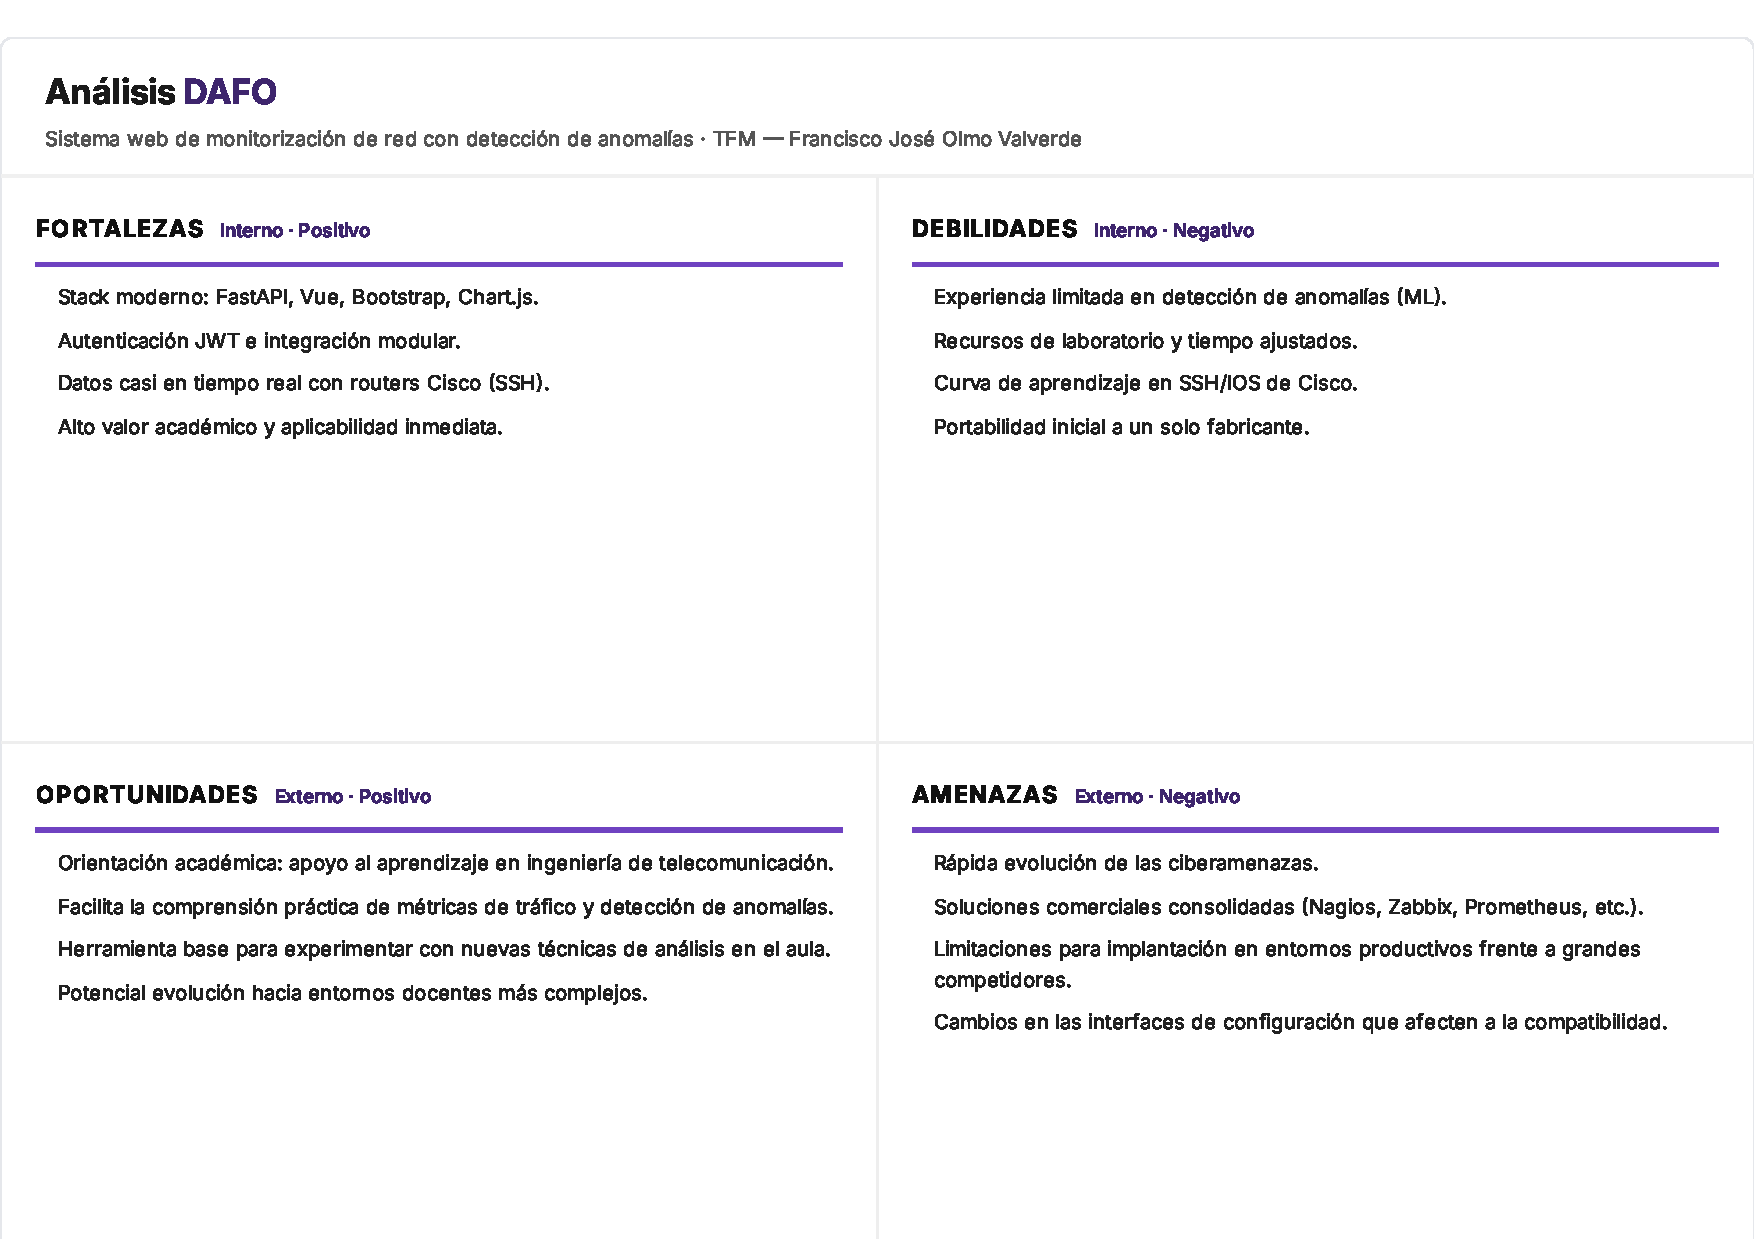
\includegraphics[height=\textwidth]{canva/DAFO.pdf}
  \caption{Análisis DAFO del proyecto}
  \label{fig:dafo}
\end{figure}
\end{landscape}